%%%%%%%%%%%%%%%%%%%%%%%%%%%%%%%%%%%%%%%%%
%  My documentation report
%  Objetive: Explain what I did and how, so someone can continue with the investigation
%
% Important note:
% Chapter heading images should have a 2:1 width:height ratio,
% e.g. 920px width and 460px height.
%
%%%%%%%%%%%%%%%%%%%%%%%%%%%%%%%%%%%%%%%%%

%----------------------------------------------------------------------------------------
%	PACKAGES AND OTHER DOCUMENT CONFIGURATIONS
%----------------------------------------------------------------------------------------

\documentclass[11pt,fleqn]{book} % Default font size and left-justified equations

\usepackage[top=3cm,bottom=3cm,left=3.2cm,right=3.2cm,headsep=10pt,letterpaper]{geometry} % Page margins

\usepackage{xcolor} % Required for specifying colors by name
\definecolor{ocre}{RGB}{52,177,201} % Define the orange color used for highlighting throughout the book

% Font Settings
\usepackage{avant} % Use the Avantgarde font for headings
%\usepackage{times} % Use the Times font for headings
\usepackage{mathptmx} % Use the Adobe Times Roman as the default text font together with math symbols from the Sym­bol, Chancery and Com­puter Modern fonts

\usepackage{microtype} % Slightly tweak font spacing for aesthetics
\usepackage[utf8]{inputenc} % Required for including letters with accents
\usepackage[T1]{fontenc} % Use 8-bit encoding that has 256 glyphs

%Tables
\usepackage{tabularx}
\usepackage{longtable,tabu}

% Bibliography
\usepackage[style=alphabetic,sorting=nyt,sortcites=true,autopunct=true,babel=hyphen,hyperref=true,abbreviate=false,backref=true,backend=biber]{biblatex}
\addbibresource{bibliography.bib} % BibTeX bibliography file
\defbibheading{bibempty}{}

%----------------------------------------------------------------------------------------
%	VARIOUS REQUIRED PACKAGES
%----------------------------------------------------------------------------------------

\usepackage{titlesec} % Allows customization of titles

\usepackage{graphicx} % Required for including pictures
\graphicspath{{Pictures/}} % Specifies the directory where pictures are stored

\usepackage{lipsum} % Inserts dummy text

\usepackage{tikz} % Required for drawing custom shapes

\usepackage[english]{babel} % English language/hyphenation

\usepackage{enumitem} % Customize lists
\setlist{nolistsep} % Reduce spacing between bullet points and numbered lists

\usepackage{booktabs} % Required for nicer horizontal rules in tables

\usepackage{eso-pic} % Required for specifying an image background in the title page

%----------------------------------------------------------------------------------------
%	MAIN TABLE OF CONTENTS
%----------------------------------------------------------------------------------------

\usepackage{titletoc} % Required for manipulating the table of contents

\contentsmargin{0cm} % Removes the default margin
% Chapter text styling
\titlecontents{chapter}[1.25cm] % Indentation
{\addvspace{15pt}\large\sffamily\bfseries} % Spacing and font options for chapters
{\color{ocre!60}\contentslabel[\Large\thecontentslabel]{1.25cm}\color{ocre}} % Chapter number
{}  
{\color{ocre!60}\normalsize\sffamily\bfseries\;\titlerule*[.5pc]{.}\;\thecontentspage} % Page number
% Section text styling
\titlecontents{section}[1.25cm] % Indentation
{\addvspace{5pt}\sffamily\bfseries} % Spacing and font options for sections
{\contentslabel[\thecontentslabel]{1.25cm}} % Section number
{}
{\sffamily\hfill\color{black}\thecontentspage} % Page number
[]
% Subsection text styling
\titlecontents{subsection}[1.25cm] % Indentation
{\addvspace{1pt}\sffamily\small} % Spacing and font options for subsections
{\contentslabel[\thecontentslabel]{1.25cm}} % Subsection number
{}
{\sffamily\;\titlerule*[.5pc]{.}\;\thecontentspage} % Page number
[] 

%----------------------------------------------------------------------------------------
%	MINI TABLE OF CONTENTS IN CHAPTER HEADS
%----------------------------------------------------------------------------------------

% Section text styling
\titlecontents{lsection}[0em] % Indendating
{\footnotesize\sffamily} % Font settings
{}
{}
{}

% Subsection text styling
\titlecontents{lsubsection}[.5em] % Indentation
{\normalfont\footnotesize\sffamily} % Font settings
{}
{}
{}
 
%----------------------------------------------------------------------------------------
%	PAGE HEADERS
%----------------------------------------------------------------------------------------

\usepackage{fancyhdr} % Required for header and footer configuration

\pagestyle{fancy}
\renewcommand{\chaptermark}[1]{\markboth{\sffamily\normalsize\bfseries\chaptername\ \thechapter.\ #1}{}} % Chapter text font settings
\renewcommand{\sectionmark}[1]{\markright{\sffamily\normalsize\thesection\hspace{5pt}#1}{}} % Section text font settings
\fancyhf{} \fancyhead[LE,RO]{\sffamily\normalsize\thepage} % Font setting for the page number in the header
\fancyhead[LO]{\rightmark} % Print the nearest section name on the left side of odd pages
\fancyhead[RE]{\leftmark} % Print the current chapter name on the right side of even pages
\renewcommand{\headrulewidth}{0.5pt} % Width of the rule under the header
\addtolength{\headheight}{2.5pt} % Increase the spacing around the header slightly
\renewcommand{\footrulewidth}{0pt} % Removes the rule in the footer
\fancypagestyle{plain}{\fancyhead{}\renewcommand{\headrulewidth}{0pt}} % Style for when a plain pagestyle is specified

% Removes the header from odd empty pages at the end of chapters
\makeatletter
\renewcommand{\cleardoublepage}{
\clearpage\ifodd\c@page\else
\hbox{}
\vspace*{\fill}
\thispagestyle{empty}
\newpage
\fi}

%----------------------------------------------------------------------------------------
%	THEOREM STYLES
%----------------------------------------------------------------------------------------

\usepackage{amsmath,amsfonts,amssymb,amsthm} % For math equations, theorems, symbols, etc

\newcommand{\intoo}[2]{\mathopen{]}#1\,;#2\mathclose{[}}
\newcommand{\ud}{\mathop{\mathrm{{}d}}\mathopen{}}
\newcommand{\intff}[2]{\mathopen{[}#1\,;#2\mathclose{]}}
\newtheorem{notation}{Notation}[chapter]

%%%%%%%%%%%%%%%%%%%%%%%%%%%%%%%%%%%%%%%%%%%%%%%%%%%%%%%%%%%%%%%%%%%%%%%%%%%
%%%%%%%%%%%%%%%%%%%% dedicated to boxed/framed environements %%%%%%%%%%%%%%
%%%%%%%%%%%%%%%%%%%%%%%%%%%%%%%%%%%%%%%%%%%%%%%%%%%%%%%%%%%%%%%%%%%%%%%%%%%
\newtheoremstyle{ocrenumbox}% % Theorem style name
{0pt}% Space above
{0pt}% Space below
{\normalfont}% % Body font
{}% Indent amount
{\small\bf\sffamily\color{ocre}}% % Theorem head font
{\;}% Punctuation after theorem head
{0.25em}% Space after theorem head
{\small\sffamily\color{ocre}\thmname{#1}\nobreakspace\thmnumber{\@ifnotempty{#1}{}\@upn{#2}}% Theorem text (e.g. Theorem 2.1)
\thmnote{\nobreakspace\the\thm@notefont\sffamily\bfseries\color{black}---\nobreakspace#3.}} % Optional theorem note
\renewcommand{\qedsymbol}{$\blacksquare$}% Optional qed square

\newtheoremstyle{blacknumex}% Theorem style name
{5pt}% Space above
{5pt}% Space below
{\normalfont}% Body font
{} % Indent amount
{\small\bf\sffamily}% Theorem head font
{\;}% Punctuation after theorem head
{0.25em}% Space after theorem head
{\small\sffamily{\tiny\ensuremath{\blacksquare}}\nobreakspace\thmname{#1}\nobreakspace\thmnumber{\@ifnotempty{#1}{}\@upn{#2}}% Theorem text (e.g. Theorem 2.1)
\thmnote{\nobreakspace\the\thm@notefont\sffamily\bfseries---\nobreakspace#3.}}% Optional theorem note

\newtheoremstyle{blacknumbox} % Theorem style name
{0pt}% Space above
{0pt}% Space below
{\normalfont}% Body font
{}% Indent amount
{\small\bf\sffamily}% Theorem head font
{\;}% Punctuation after theorem head
{0.25em}% Space after theorem head
{\small\sffamily\thmname{#1}\nobreakspace\thmnumber{\@ifnotempty{#1}{}\@upn{#2}}% Theorem text (e.g. Theorem 2.1)
\thmnote{\nobreakspace\the\thm@notefont\sffamily\bfseries---\nobreakspace#3.}}% Optional theorem note

%%%%%%%%%%%%%%%%%%%%%%%%%%%%%%%%%%%%%%%%%%%%%%%%%%%%%%%%%%%%%%%%%%%%%%%%%%%
%%%%%%%%%%%%% dedicated to non-boxed/non-framed environements %%%%%%%%%%%%%
%%%%%%%%%%%%%%%%%%%%%%%%%%%%%%%%%%%%%%%%%%%%%%%%%%%%%%%%%%%%%%%%%%%%%%%%%%%
\newtheoremstyle{ocrenum}% % Theorem style name
{5pt}% Space above
{5pt}% Space below
{\normalfont}% % Body font
{}% Indent amount
{\small\bf\sffamily\color{ocre}}% % Theorem head font
{\;}% Punctuation after theorem head
{0.25em}% Space after theorem head
{\small\sffamily\color{ocre}\thmname{#1}\nobreakspace\thmnumber{\@ifnotempty{#1}{}\@upn{#2}}% Theorem text (e.g. Theorem 2.1)
\thmnote{\nobreakspace\the\thm@notefont\sffamily\bfseries\color{black}---\nobreakspace#3.}} % Optional theorem note
\renewcommand{\qedsymbol}{$\blacksquare$}% Optional qed square
\makeatother

% Defines the theorem text style for each type of theorem to one of the three styles above
\newcounter{dummy} 
\numberwithin{dummy}{section}
\theoremstyle{ocrenumbox}
\newtheorem{theoremeT}[dummy]{Theorem}
\newtheorem{problem}{Problem}[chapter]
\newtheorem{exerciseT}{Exercise}[chapter]
\theoremstyle{blacknumex}
\newtheorem{exampleT}{Example}[chapter]
\theoremstyle{blacknumbox}
\newtheorem{vocabulary}{Vocabulary}[chapter]
\newtheorem{definitionT}{Definition}[section]
\newtheorem{corollaryT}[dummy]{Corollary}
\theoremstyle{ocrenum}
\newtheorem{proposition}[dummy]{Proposition}

%----------------------------------------------------------------------------------------
%	DEFINITION OF COLORED BOXES
%----------------------------------------------------------------------------------------

\RequirePackage[framemethod=default]{mdframed} % Required for creating the theorem, definition, exercise and corollary boxes

% Theorem box
\newmdenv[skipabove=7pt,
skipbelow=7pt,
backgroundcolor=black!5,
linecolor=ocre,
innerleftmargin=5pt,
innerrightmargin=5pt,
innertopmargin=5pt,
leftmargin=0cm,
rightmargin=0cm,
innerbottommargin=5pt]{tBox}

% Exercise box	  
\newmdenv[skipabove=7pt,
skipbelow=7pt,
rightline=false,
leftline=true,
topline=false,
bottomline=false,
backgroundcolor=ocre!10,
linecolor=ocre,
innerleftmargin=5pt,
innerrightmargin=5pt,
innertopmargin=5pt,
innerbottommargin=5pt,
leftmargin=0cm,
rightmargin=0cm,
linewidth=4pt]{eBox}	

% Definition box
\newmdenv[skipabove=7pt,
skipbelow=7pt,
rightline=false,
leftline=true,
topline=false,
bottomline=false,
linecolor=ocre,
innerleftmargin=5pt,
innerrightmargin=5pt,
innertopmargin=0pt,
leftmargin=0cm,
rightmargin=0cm,
linewidth=4pt,
innerbottommargin=0pt]{dBox}	

% Corollary box
\newmdenv[skipabove=7pt,
skipbelow=7pt,
rightline=false,
leftline=true,
topline=false,
bottomline=false,
linecolor=gray,
backgroundcolor=black!5,
innerleftmargin=5pt,
innerrightmargin=5pt,
innertopmargin=5pt,
leftmargin=0cm,
rightmargin=0cm,
linewidth=4pt,
innerbottommargin=5pt]{cBox}

% Creates an environment for each type of theorem and assigns it a theorem text style from the "Theorem Styles" section above and a colored box from above
\newenvironment{theorem}{\begin{tBox}\begin{theoremeT}}{\end{theoremeT}\end{tBox}}
\newenvironment{exercise}{\begin{eBox}\begin{exerciseT}}{\hfill{\color{ocre}\tiny\ensuremath{\blacksquare}}\end{exerciseT}\end{eBox}}				  
\newenvironment{definition}{\begin{dBox}\begin{definitionT}}{\end{definitionT}\end{dBox}}	
\newenvironment{example}{\begin{exampleT}}{\hfill{\tiny\ensuremath{\blacksquare}}\end{exampleT}}		
\newenvironment{corollary}{\begin{cBox}\begin{corollaryT}}{\end{corollaryT}\end{cBox}}	

%----------------------------------------------------------------------------------------
%	REMARK ENVIRONMENT
%----------------------------------------------------------------------------------------

\newenvironment{remark}{\par\vspace{10pt}\small % Vertical white space above the remark and smaller font size
\begin{list}{}{
\leftmargin=35pt % Indentation on the left
\rightmargin=25pt}\item\ignorespaces % Indentation on the right
\makebox[-2.5pt]{\begin{tikzpicture}[overlay]
\node[draw=ocre!60,line width=1pt,circle,fill=ocre!25,font=\sffamily\bfseries,inner sep=2pt,outer sep=0pt] at (-15pt,0pt){\textcolor{ocre}{R}};\end{tikzpicture}} % Orange R in a circle
\advance\baselineskip -1pt}{\end{list}\vskip5pt} % Tighter line spacing and white space after remark

%----------------------------------------------------------------------------------------
%	SECTION NUMBERING IN THE MARGIN
%----------------------------------------------------------------------------------------

\makeatletter
\renewcommand{\@seccntformat}[1]{\llap{\textcolor{ocre}{\csname the#1\endcsname}\hspace{1em}}}                    
\renewcommand{\section}{\@startsection{section}{1}{\z@}
{-4ex \@plus -1ex \@minus -.4ex}
{1ex \@plus.2ex }
{\normalfont\large\sffamily\bfseries}}
\renewcommand{\subsection}{\@startsection {subsection}{2}{\z@}
{-3ex \@plus -0.1ex \@minus -.4ex}
{0.5ex \@plus.2ex }
{\normalfont\sffamily\bfseries}}
\renewcommand{\subsubsection}{\@startsection {subsubsection}{3}{\z@}
{-2ex \@plus -0.1ex \@minus -.2ex}
{.2ex \@plus.2ex }
{\normalfont\small\sffamily\bfseries}}                        
\renewcommand\paragraph{\@startsection{paragraph}{4}{\z@}
{-2ex \@plus-.2ex \@minus .2ex}
{.1ex}
{\normalfont\small\sffamily\bfseries}}

%----------------------------------------------------------------------------------------
%	HYPERLINKS IN THE DOCUMENTS
%----------------------------------------------------------------------------------------

% For an unclear reason, the package should be loaded now and not later
\usepackage{hyperref}
\hypersetup{hidelinks,backref=true,pagebackref=true,hyperindex=true,colorlinks=false,breaklinks=true,urlcolor= ocre,bookmarks=true,bookmarksopen=false,pdftitle={Title},pdfauthor={Author}}

%----------------------------------------------------------------------------------------
%	CHAPTER HEADINGS
%----------------------------------------------------------------------------------------

% The set-up below should be (sadly) manually adapted to the overall margin page septup controlled by the geometry package loaded in the main.tex document. It is possible to implement below the dimensions used in the goemetry package (top,bottom,left,right)... TO BE DONE

\newcommand{\thechapterimage}{}
\newcommand{\chapterimage}[1]{\renewcommand{\thechapterimage}{#1}}

% Numbered chapters with mini tableofcontents
\def\thechapter{\arabic{chapter}}
\def\@makechapterhead#1{
\thispagestyle{empty}
{\centering \normalfont\sffamily
\ifnum \c@secnumdepth >\m@ne
\if@mainmatter
\startcontents
\begin{tikzpicture}[remember picture,overlay]
\node at (current page.north west)
{\begin{tikzpicture}[remember picture,overlay]
\node[anchor=north west,inner sep=0pt] at (0,0) {\includegraphics[width=\paperwidth]{\thechapterimage}};
%%%%%%%%%%%%%%%%%%%%%%%%%%%%%%%%%%%%%%%%%%%%%%%%%%%%%%%%%%%%%%%%%%%%%%%%%%%%%%%%%%%%%
% Commenting the 3 lines below removes the small contents box in the chapter heading
%\fill[color=ocre!10!white,opacity=.6] (1cm,0) rectangle (8cm,-7cm);
%\node[anchor=north west] at (1.1cm,.35cm) {\parbox[t][8cm][t]{6.5cm}{\huge\bfseries\flushleft \printcontents{l}{1}{\setcounter{tocdepth}{2}}}};
\draw[anchor=west] (5cm,-9cm) node [rounded corners=20pt,fill=ocre!10!white,text opacity=1,draw=ocre,draw opacity=1,line width=1.5pt,fill opacity=.6,inner sep=12pt]{\huge\sffamily\bfseries\textcolor{black}{\thechapter. #1\strut\makebox[22cm]{}}};
%%%%%%%%%%%%%%%%%%%%%%%%%%%%%%%%%%%%%%%%%%%%%%%%%%%%%%%%%%%%%%%%%%%%%%%%%%%%%%%%%%%%%
\end{tikzpicture}};
\end{tikzpicture}}
\par\vspace*{230\p@}
\fi
\fi}

% Unnumbered chapters without mini tableofcontents (could be added though) 
\def\@makeschapterhead#1{
\thispagestyle{empty}
{\centering \normalfont\sffamily
\ifnum \c@secnumdepth >\m@ne
\if@mainmatter
\begin{tikzpicture}[remember picture,overlay]
\node at (current page.north west)
{\begin{tikzpicture}[remember picture,overlay]
\node[anchor=north west,inner sep=0pt] at (0,0) {\includegraphics[width=\paperwidth]{\thechapterimage}};
\draw[anchor=west] (5cm,-9cm) node [rounded corners=20pt,fill=ocre!10!white,fill opacity=.6,inner sep=12pt,text opacity=1,draw=ocre,draw opacity=1,line width=1.5pt]{\huge\sffamily\bfseries\textcolor{black}{#1\strut\makebox[22cm]{}}};
\end{tikzpicture}};
\end{tikzpicture}}
\par\vspace*{230\p@}
\fi
\fi
}
\makeatother % Insert the commands.tex file which contains the majority of the structure behind the template

\begin{document}

%----------------------------------------------------------------------------------------
%	TITLE PAGE
%----------------------------------------------------------------------------------------

\begingroup
\thispagestyle{empty}
\AddToShipoutPicture*{\put(0,0){\includegraphics[scale=1.25]{cover}}} % Image background
\centering
\vspace*{4cm}
\par\normalfont\fontsize{35}{35}\sffamily\selectfont
\textbf{\color{white}Data Mining for Bee Micro-sensors}\\
{\Huge\color{white} Laboratorio Nacional de Análisis y Síntesis Ecológica}\par % Book title
\vspace*{0.2cm}
%Add all the collaborators
%{\LARGE\color{white} Laboratorio Nacional de Análisis y Síntesis Ecológica}\par % Author name
{\LARGE\color{white} Framework Developed by:\\ Ulises Olivares, Gloria Ruiz, Maria J. Aguilar, Oliverio Delgado, Francisco J. Balvino, Mauricio Quesada }\par % Author name
\endgroup

%----------------------------------------------------------------------------------------
%	COPYRIGHT PAGE
%----------------------------------------------------------------------------------------

\newpage
~\vfill
\thispagestyle{empty}

%\noindent Copyright \copyright\ 2014 Andrea Hidalgo\\ % Copyright notice

\noindent \textsc{High Performance Computing applied to biological sciences, Universidad Nacional Autónoma de México - Escuela Nacional de de Estudios Superiores Unidad Morelia - Laboratorio Nacional de Análisis y Síntesis Ecológica }\\

\noindent  This work was supported by grants from Consejo Nacional de Ciencia y Tecnología (CONACyT: Laboratorio Nacional de Análisis y Síntesis Ecológica U-3-2015-2-250996, CONACYT and CONACyT: Propuesta para eldesarrollo de una infraestructura tecnológica para lacreación de repositorios masivos de datos biológicos con fines de conservación y análisis de información I0028-2015-02-271432, CONACYT).\\ % License information

\noindent \textit{First release, April 2017} % Printing/edition date

%----------------------------------------------------------------------------------------
%	TABLE OF CONTENTS
%----------------------------------------------------------------------------------------

\chapterimage{head1.jpg} % Table of contents heading image

\pagestyle{empty} % No headers

\tableofcontents % Print the table of contents itself

%\cleardoublepage % Forces the first chapter to start on an odd page so it's on the right

\pagestyle{fancy} % Print headers again

%----------------------------------------------------------------------------------------
%	CHAPTER 1
%----------------------------------------------------------------------------------------
\chapterimage{head2.jpg} % Chapter heading image

\chapter{Introduction}

%INSERT_CONTENT_HERE
\normalsize%
\section*{Introduction}%
The main propose of this document  is to show a concise report about the activity of bees and behavior in a specific period of time. This report also shows a complete analysis of the most active hours.\newline%
\newline%
Tis report corresponds to a period of time of 123 day(s). From 2016{-}07{-}02 to 2016{-}12{-}02. During this period of time, a total amount of 18653 lectures were registered from 156 different bees. There exist a total of 26 non{-}active days. We define an 'active day' if there is more than one observation. (see Figure1.1).\newline%
\newline%
%


\begin{figure}[h!]%
\centering%
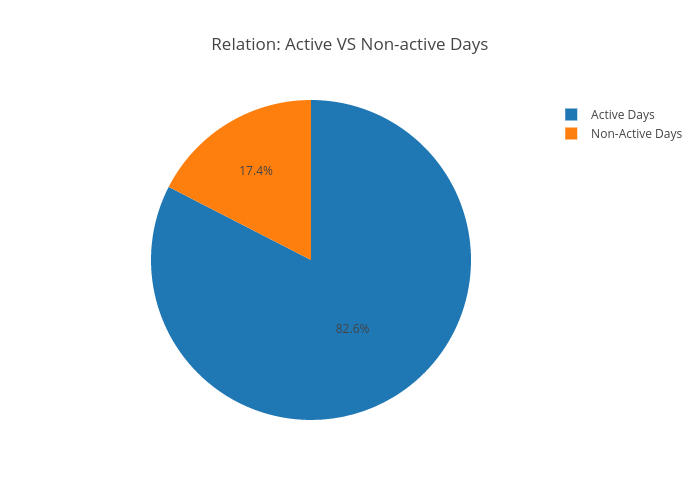
\includegraphics[width=315px]{chartNumLectures.png}%
\caption{Days with and without Empty Reads}%
\end{figure}


\chapterimage{head3.jpg} % Chapter heading image
\chapter{Analysis of Raw Data}
\normalsize%
\subsection*{Activity Per Day of Raw Data}%
This section addresses the analysis of raw data. Which implies that this date is presented without filters or a data preprocessing step to clean the data. This section presents severalgraphs which reflects the behavior of a beehive during a specific period of time.%


\begin{figure}[h!]%
\centering%
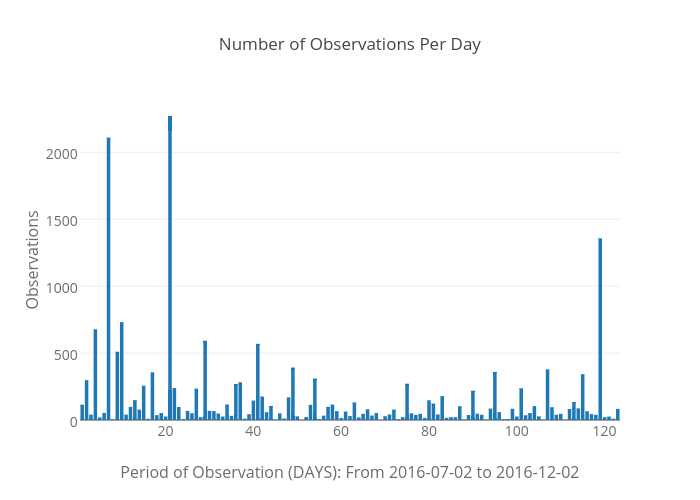
\includegraphics[width=400px]{observationsPerdayUnclean.png}%
\caption{Number of Observations per Day}%
\end{figure}

%
\begin{longtabu}{| c | c | c | c |}%
\hline%
Day&Date&\# Observations&\# Bees per day\\%
\hline%
1&2016{-}07{-}02&1&1\\%
\hline%
2&2016{-}07{-}03&1&1\\%
\hline%
3&2016{-}07{-}08&50&8\\%
\hline%
4&2016{-}07{-}09&145&11\\%
\hline%
5&2016{-}07{-}10&115&10\\%
\hline%
6&2016{-}07{-}11&50&7\\%
\hline%
7&2016{-}07{-}12&21&5\\%
\hline%
8&2016{-}07{-}13&26&7\\%
\hline%
9&2016{-}07{-}14&65&4\\%
\hline%
10&2016{-}07{-}15&731&14\\%
\hline%
11&2016{-}07{-}16&510&11\\%
\hline%
12&2016{-}07{-}17&68&5\\%
\hline%
13&2016{-}07{-}18&43&3\\%
\hline%
14&2016{-}07{-}19&32&3\\%
\hline%
15&2016{-}07{-}20&33&3\\%
\hline%
16&2016{-}07{-}21&16&3\\%
\hline%
17&2016{-}07{-}22&6&2\\%
\hline%
18&2016{-}07{-}23&342&16\\%
\hline%
19&2016{-}07{-}24&256&12\\%
\hline%
20&2016{-}07{-}25&66&8\\%
\hline%
21&2016{-}07{-}26&105&7\\%
\hline%
22&2016{-}07{-}27&29&5\\%
\hline%
23&2016{-}07{-}28&21&5\\%
\hline%
24&2016{-}07{-}29&37&6\\%
\hline%
25&2016{-}07{-}30&27&4\\%
\hline%
26&2016{-}07{-}31&26&4\\%
\hline%
27&2016{-}08{-}01&41&5\\%
\hline%
28&2016{-}08{-}02&39&5\\%
\hline%
29&2016{-}08{-}03&35&5\\%
\hline%
30&2016{-}08{-}04&21&5\\%
\hline%
31&2016{-}08{-}05&98&5\\%
\hline%
32&2016{-}08{-}06&15&6\\%
\hline%
33&2016{-}08{-}07&175&15\\%
\hline%
34&2016{-}08{-}08&147&13\\%
\hline%
35&2016{-}08{-}09&131&11\\%
\hline%
36&2016{-}08{-}10&82&8\\%
\hline%
37&2016{-}08{-}11&85&7\\%
\hline%
38&2016{-}08{-}12&239&9\\%
\hline%
39&2016{-}08{-}13&53&8\\%
\hline%
40&2016{-}08{-}14&113&7\\%
\hline%
41&2016{-}08{-}15&269&12\\%
\hline%
42&2016{-}08{-}16&271&14\\%
\hline%
43&2016{-}08{-}17&98&7\\%
\hline%
44&2016{-}08{-}18&378&12\\%
\hline%
45&2016{-}08{-}19&219&8\\%
\hline%
46&2016{-}08{-}20&356&8\\%
\hline%
47&2016{-}08{-}21&83&7\\%
\hline%
48&2016{-}08{-}22&49&7\\%
\hline%
49&2016{-}08{-}23&48&4\\%
\hline%
50&2016{-}08{-}24&52&5\\%
\hline%
51&2016{-}08{-}25&27&4\\%
\hline%
52&2016{-}08{-}26&84&6\\%
\hline%
53&2016{-}09{-}20&77&3\\%
\hline%
54&2016{-}09{-}21&68&2\\%
\hline%
55&2016{-}09{-}22&104&3\\%
\hline%
56&2016{-}09{-}23&21&2\\%
\hline%
57&2016{-}09{-}24&5&1\\%
\hline%
58&2016{-}09{-}25&4&1\\%
\hline%
59&2016{-}09{-}26&10&1\\%
\hline%
60&2016{-}09{-}27&6&1\\%
\hline%
61&2016{-}09{-}28&4&1\\%
\hline%
62&2016{-}09{-}29&7&1\\%
\hline%
63&2016{-}09{-}30&7&1\\%
\hline%
64&2016{-}10{-}01&9&1\\%
\hline%
65&2016{-}10{-}02&10&1\\%
\hline%
66&2016{-}10{-}03&3&1\\%
\hline%
67&2016{-}10{-}04&3&2\\%
\hline%
68&2016{-}10{-}07&3&1\\%
\hline%
69&2016{-}10{-}09&2271&14\\%
\hline%
70&2016{-}10{-}10&19&7\\%
\hline%
71&2016{-}10{-}11&2&2\\%
\hline%
72&2016{-}10{-}12&237&7\\%
\hline%
73&2016{-}10{-}13&21&3\\%
\hline%
74&2016{-}10{-}14&28&4\\%
\hline%
75&2016{-}10{-}15&22&6\\%
\hline%
76&2016{-}10{-}16&569&3\\%
\hline%
77&2016{-}10{-}17&234&7\\%
\hline%
78&2016{-}10{-}18&40&6\\%
\hline%
79&2016{-}10{-}19&44&5\\%
\hline%
80&2016{-}10{-}20&39&3\\%
\hline%
81&2016{-}10{-}21&47&5\\%
\hline%
82&2016{-}10{-}22&38&4\\%
\hline%
83&2016{-}10{-}23&66&4\\%
\hline%
84&2016{-}10{-}24&169&3\\%
\hline%
85&2016{-}10{-}25&116&3\\%
\hline%
86&2016{-}10{-}26&52&3\\%
\hline%
87&2016{-}10{-}27&298&5\\%
\hline%
88&2016{-}10{-}28&87&7\\%
\hline%
89&2016{-}10{-}29&59&5\\%
\hline%
90&2016{-}10{-}30&41&6\\%
\hline%
91&2016{-}10{-}31&46&5\\%
\hline%
92&2016{-}11{-}01&95&6\\%
\hline%
93&2016{-}11{-}02&114&7\\%
\hline%
94&2016{-}11{-}03&36&7\\%
\hline%
95&2016{-}11{-}04&26&5\\%
\hline%
96&2016{-}11{-}05&11&4\\%
\hline%
97&2016{-}11{-}06&19&6\\%
\hline%
98&2016{-}11{-}07&123&6\\%
\hline%
99&2016{-}11{-}08&359&14\\%
\hline%
100&2016{-}11{-}09&134&8\\%
\hline%
101&2016{-}11{-}10&2110&6\\%
\hline%
102&2016{-}11{-}11&97&7\\%
\hline%
103&2016{-}11{-}12&282&7\\%
\hline%
104&2016{-}11{-}13&309&5\\%
\hline%
105&2016{-}11{-}14&78&7\\%
\hline%
106&2016{-}11{-}15&103&6\\%
\hline%
107&2016{-}11{-}16&51&6\\%
\hline%
108&2016{-}11{-}17&1357&5\\%
\hline%
109&2016{-}11{-}18&148&6\\%
\hline%
110&2016{-}11{-}19&592&5\\%
\hline%
111&2016{-}11{-}20&58&6\\%
\hline%
112&2016{-}11{-}21&63&5\\%
\hline%
113&2016{-}11{-}22&46&6\\%
\hline%
114&2016{-}11{-}23&39&5\\%
\hline%
115&2016{-}11{-}24&46&5\\%
\hline%
116&2016{-}11{-}25&40&5\\%
\hline%
117&2016{-}11{-}26&26&5\\%
\hline%
118&2016{-}11{-}27&31&3\\%
\hline%
119&2016{-}11{-}28&392&3\\%
\hline%
120&2016{-}11{-}29&80&4\\%
\hline%
121&2016{-}11{-}30&179&4\\%
\hline%
122&2016{-}12{-}01&16&3\\%
\hline%
123&2016{-}12{-}02&677&2\\%
\hline%
\hline%
{-}{-}&Average&151&5\\%
\hline%
\hline%
\end{longtabu}

%
\subsection*{Bee Life Cycle}%
In this section is analyzed the Life Cycle of each bee in the hive%
\begin{longtabu}{| c | c | c |}%
\hline%
\hline%
Register&Bee ID&Life Cycle in Days\\%
\hline%
\hline%
1&0004&1\\%
\hline%
2&0005&1\\%
\hline%
3&0006&1\\%
\hline%
4&0016&1\\%
\hline%
5&0023&1\\%
\hline%
6&0024&5\\%
\hline%
7&0027&1\\%
\hline%
8&0029&8\\%
\hline%
9&0031&1\\%
\hline%
10&0053&5\\%
\hline%
11&0055&1\\%
\hline%
12&0056&1\\%
\hline%
13&0060&1\\%
\hline%
14&0061&1\\%
\hline%
15&0062&1\\%
\hline%
16&0063&6\\%
\hline%
17&0064&1\\%
\hline%
18&0068&16\\%
\hline%
19&0071&1\\%
\hline%
20&0075&5\\%
\hline%
21&0077&18\\%
\hline%
22&0079&122\\%
\hline%
23&0081&1\\%
\hline%
24&0082&1\\%
\hline%
25&0083&1\\%
\hline%
26&0087&2\\%
\hline%
27&0090&3\\%
\hline%
28&0093&1\\%
\hline%
29&0094&1\\%
\hline%
30&0095&1\\%
\hline%
31&0096&1\\%
\hline%
32&0103&1\\%
\hline%
33&0108&17\\%
\hline%
34&0112&1\\%
\hline%
35&0118&1\\%
\hline%
36&0130&23\\%
\hline%
37&0137&5\\%
\hline%
38&0145&3\\%
\hline%
39&0146&2\\%
\hline%
40&0153&3\\%
\hline%
41&0154&1\\%
\hline%
42&0155&1\\%
\hline%
43&0156&2\\%
\hline%
44&0157&2\\%
\hline%
45&0158&1\\%
\hline%
46&0162&3\\%
\hline%
47&0165&2\\%
\hline%
48&0174&1\\%
\hline%
49&0188&7\\%
\hline%
50&0189&2\\%
\hline%
51&0194&1\\%
\hline%
52&0203&1\\%
\hline%
53&0207&1\\%
\hline%
54&0208&2\\%
\hline%
55&0212&16\\%
\hline%
56&0213&27\\%
\hline%
57&0215&1\\%
\hline%
58&0218&1\\%
\hline%
59&0220&1\\%
\hline%
60&0223&117\\%
\hline%
61&0234&18\\%
\hline%
62&0235&2\\%
\hline%
63&0237&1\\%
\hline%
64&0250&1\\%
\hline%
65&0256&20\\%
\hline%
66&0257&3\\%
\hline%
67&0258&1\\%
\hline%
68&0261&1\\%
\hline%
69&0264&14\\%
\hline%
70&0266&20\\%
\hline%
71&0267&20\\%
\hline%
72&0270&1\\%
\hline%
73&0273&3\\%
\hline%
74&0276&9\\%
\hline%
75&0278&1\\%
\hline%
76&0282&1\\%
\hline%
77&0283&6\\%
\hline%
78&0286&1\\%
\hline%
79&0287&1\\%
\hline%
80&0290&14\\%
\hline%
81&0292&4\\%
\hline%
82&0295&1\\%
\hline%
83&0296&1\\%
\hline%
84&0304&1\\%
\hline%
85&0307&3\\%
\hline%
86&0309&1\\%
\hline%
87&0311&5\\%
\hline%
88&0312&1\\%
\hline%
89&0314&1\\%
\hline%
90&0315&1\\%
\hline%
91&0316&3\\%
\hline%
92&0318&1\\%
\hline%
93&0319&1\\%
\hline%
94&0321&1\\%
\hline%
95&0324&1\\%
\hline%
96&0327&1\\%
\hline%
97&0330&6\\%
\hline%
98&0331&1\\%
\hline%
99&0332&1\\%
\hline%
100&0333&1\\%
\hline%
101&0336&1\\%
\hline%
102&0340&1\\%
\hline%
103&0341&11\\%
\hline%
104&0342&7\\%
\hline%
105&0354&1\\%
\hline%
106&0383&1\\%
\hline%
107&0391&1\\%
\hline%
108&0431&1\\%
\hline%
109&0483&1\\%
\hline%
110&0484&4\\%
\hline%
111&0488&1\\%
\hline%
112&0498&1\\%
\hline%
113&0528&1\\%
\hline%
114&0544&15\\%
\hline%
115&0546&1\\%
\hline%
116&0551&1\\%
\hline%
117&0553&27\\%
\hline%
118&0568&1\\%
\hline%
119&0569&1\\%
\hline%
120&0595&1\\%
\hline%
121&0598&1\\%
\hline%
122&0604&1\\%
\hline%
123&0605&1\\%
\hline%
124&0608&4\\%
\hline%
125&0610&27\\%
\hline%
126&0612&2\\%
\hline%
127&0616&9\\%
\hline%
128&0626&1\\%
\hline%
129&0627&1\\%
\hline%
130&0634&1\\%
\hline%
131&0636&22\\%
\hline%
132&0642&2\\%
\hline%
133&0643&13\\%
\hline%
134&0652&34\\%
\hline%
135&0668&1\\%
\hline%
136&0672&1\\%
\hline%
137&0674&1\\%
\hline%
138&0675&10\\%
\hline%
139&0676&18\\%
\hline%
140&0678&15\\%
\hline%
141&0683&2\\%
\hline%
142&0694&1\\%
\hline%
143&0697&1\\%
\hline%
144&0701&1\\%
\hline%
145&0711&1\\%
\hline%
146&0717&25\\%
\hline%
147&0724&24\\%
\hline%
148&0735&18\\%
\hline%
149&0738&18\\%
\hline%
150&0744&1\\%
\hline%
151&0746&2\\%
\hline%
152&0747&3\\%
\hline%
153&0754&1\\%
\hline%
154&0777&1\\%
\hline%
155&0795&1\\%
\hline%
156&0137&1\\%
\hline%
\hline%
{-}{-}&Average&6\\%
\hline%
\hline%
\end{longtabu}%


\begin{figure}[h!]%
\centering%
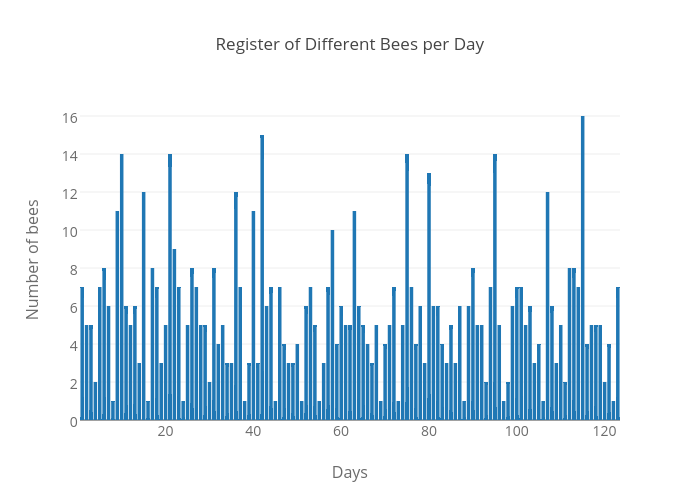
\includegraphics[width=400px]{differentBeesPerdayUnclean.png}%
\caption{Different Bees Per Day}%
\end{figure}

%


\begin{figure}[h!]%
\centering%
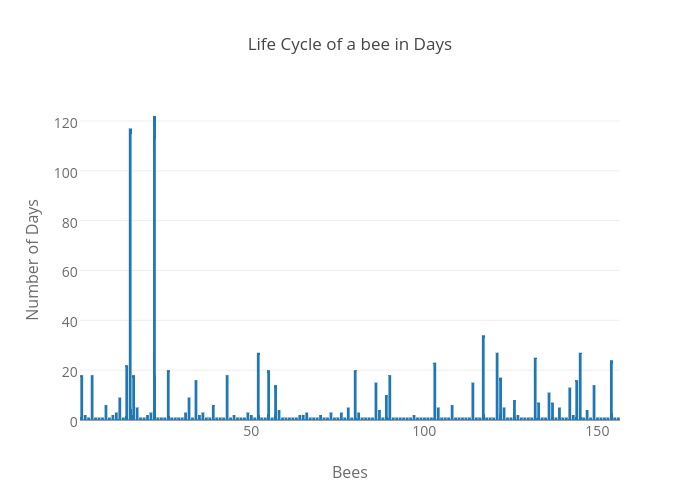
\includegraphics[width=400px]{beeLifeCycleUnclean.png}%
\caption{Bee Life cycle in days}%
\end{figure}

%


\begin{figure}[h!]%
\centering%
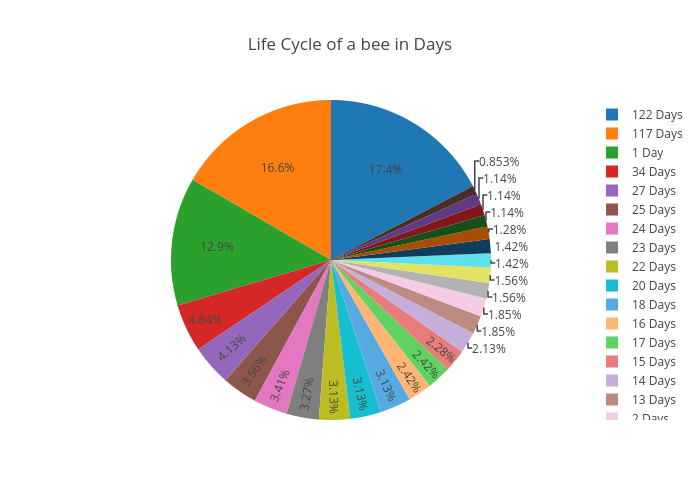
\includegraphics[width=400px]{pieBeeLifeCycleUnclean.png}%
\caption{Bee Life cycle in days}%
\end{figure}

%
\subsection*{Analysis of Activity per Hour}%


\begin{figure}[h!]%
\centering%
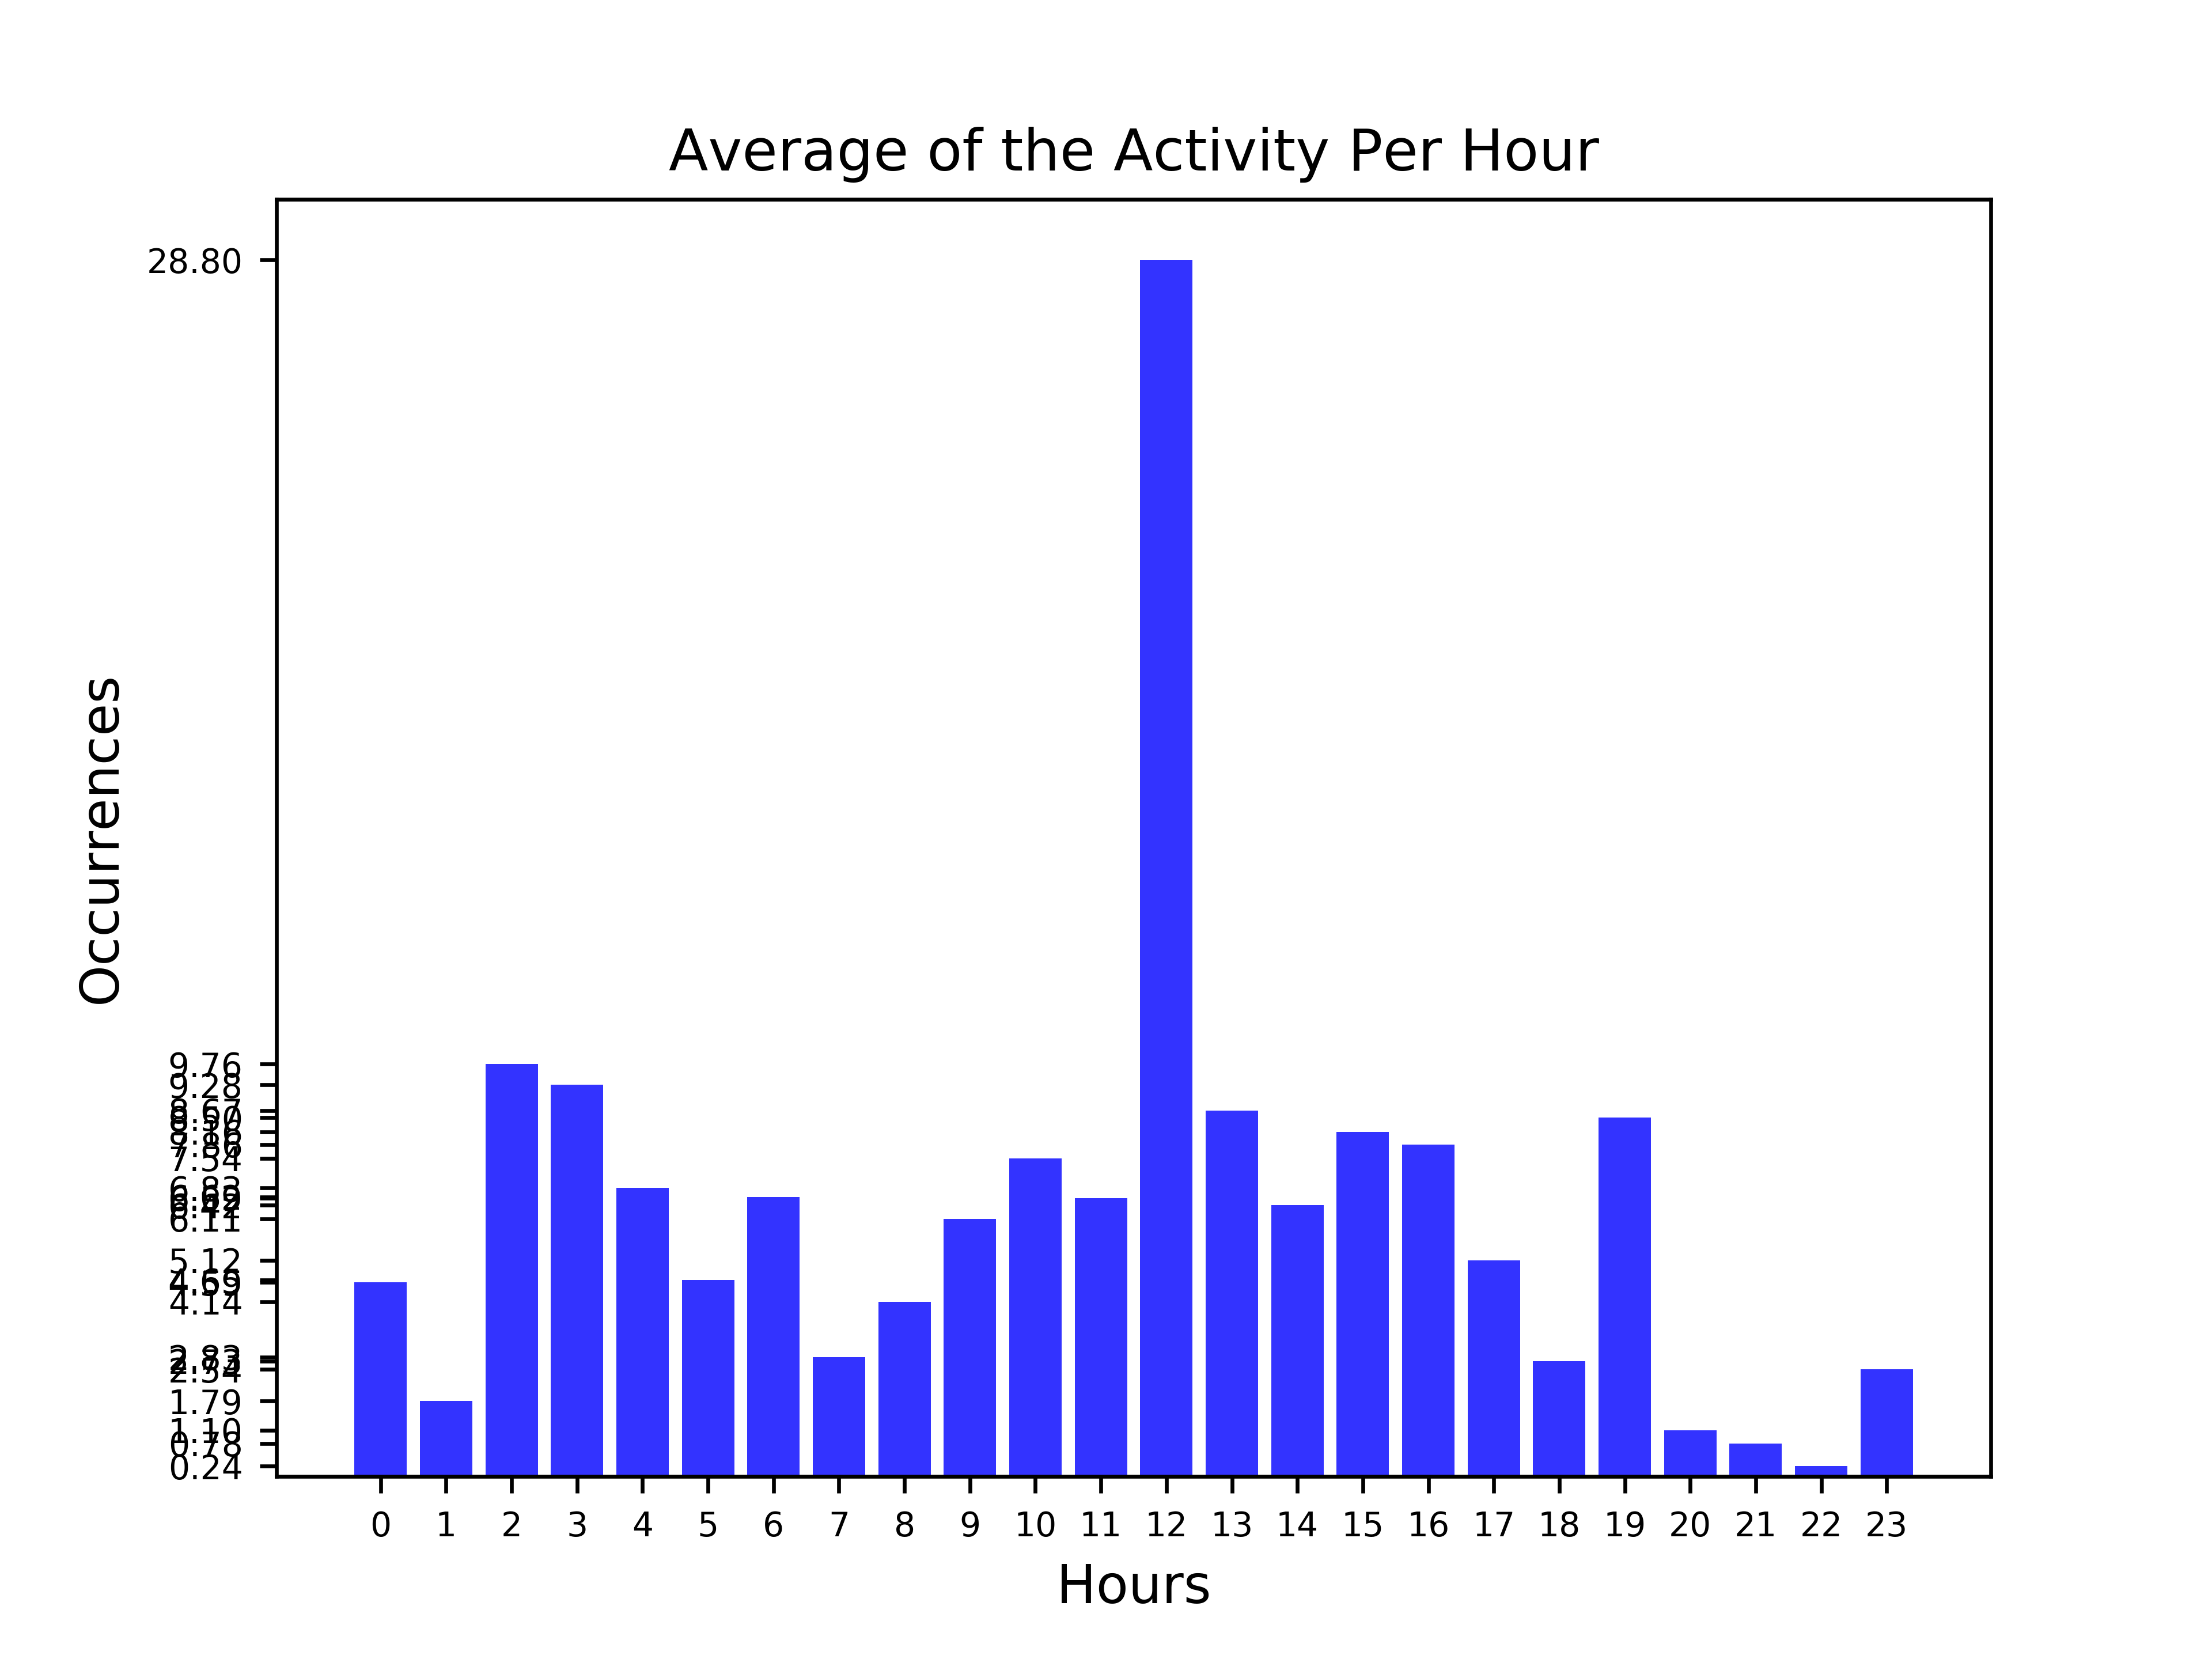
\includegraphics[width=400px]{histogramUnclean.png}%
\caption{Histogram of frequencies per hour}%
\end{figure}

%


\begin{figure}[h!]%
\centering%
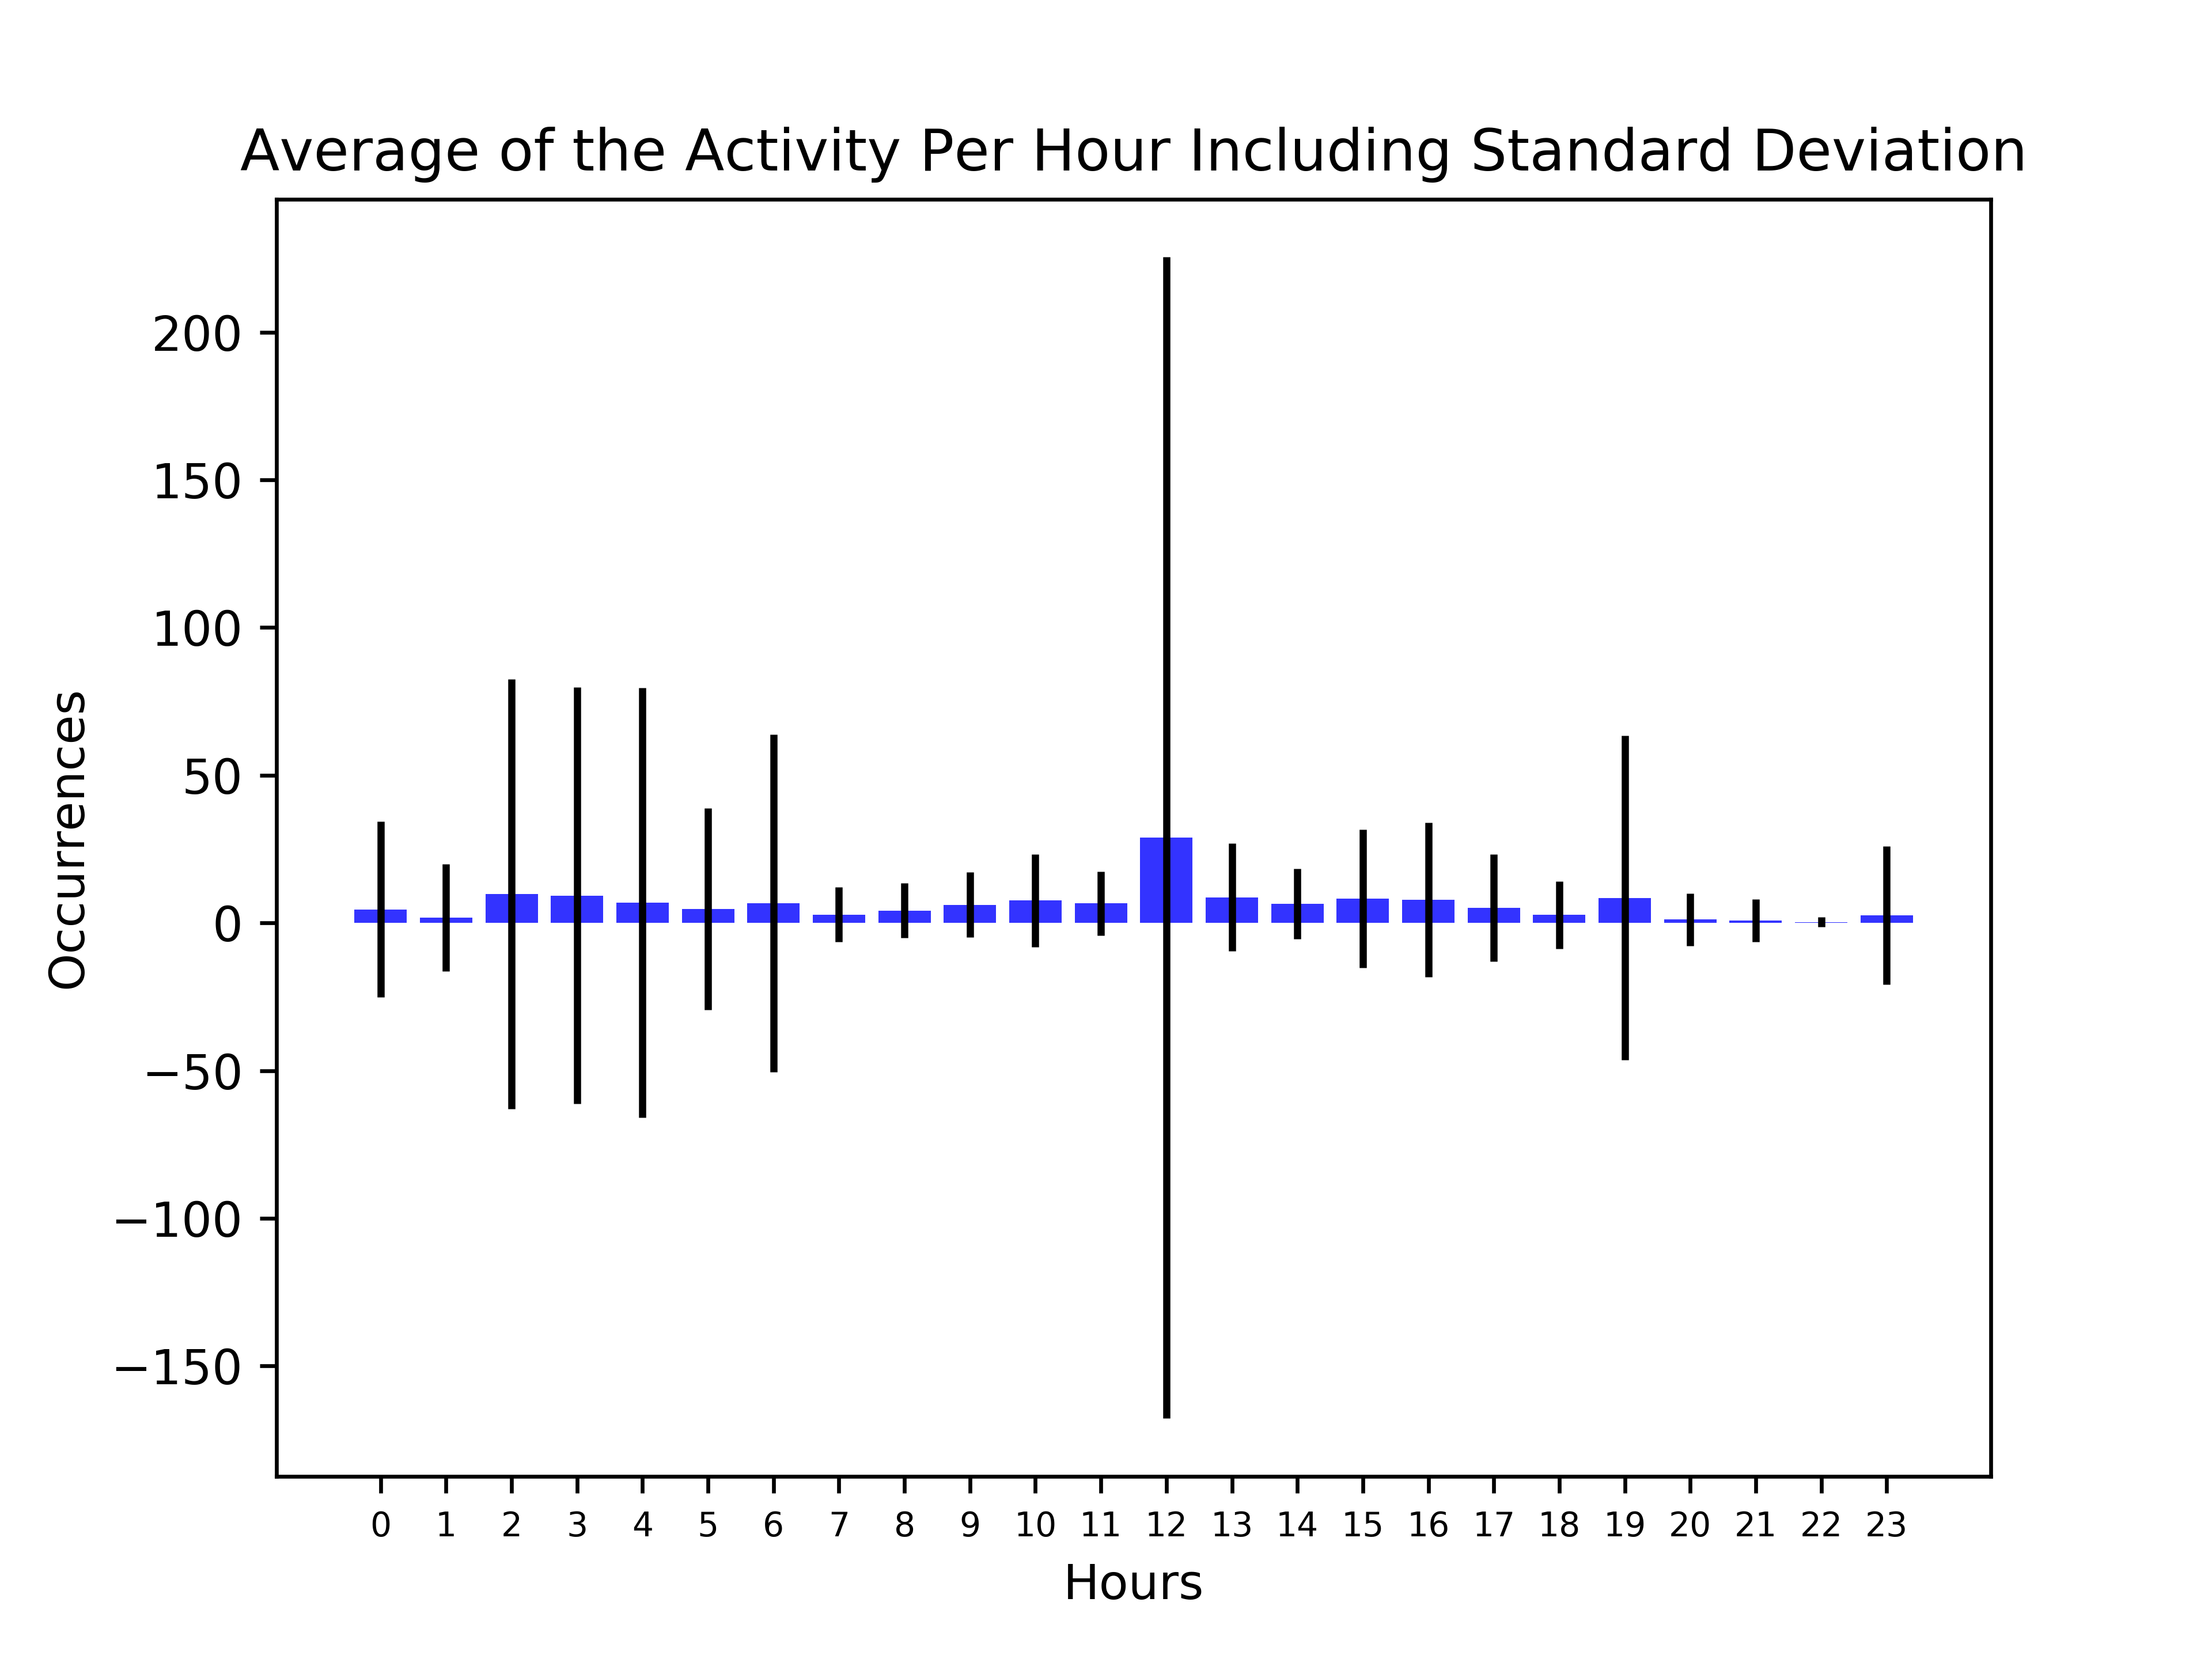
\includegraphics[width=400px]{histogramStdUnclean.png}%
\caption{Histogram of frequencies per hour. It includes standard deviation}%
\end{figure}


\chapterimage{head4.jpg} % Chapter heading image
\chapter{Analysis of Clean Data}
\normalsize%
\subsection*{Activity Per Day of Clean Data}%
In this section is presented an analysis of input data. During this analysis some filters were applied. One of these filters is the definition of a threshold which removes all the observations that fall in a period of time less than 60 seconds. This preprocessing step tends to  remove all the lost chips which generated unnecessary and repeated registers %


\begin{figure}[h!]%
\centering%
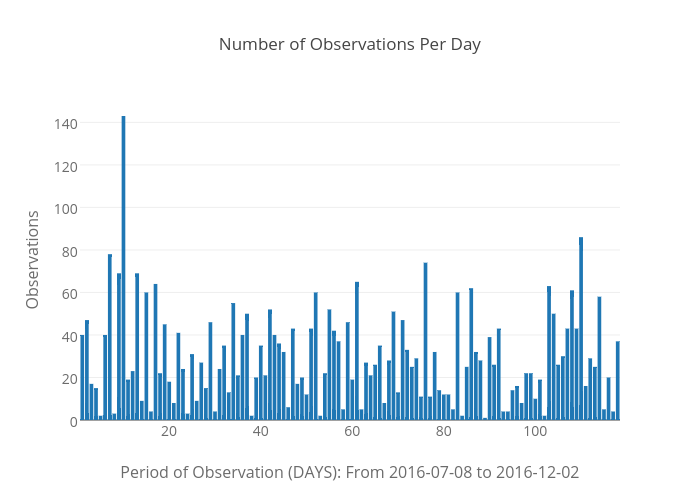
\includegraphics[width=400px]{observationsPerdayClean.png}%
\caption{Number of Observations per Day}%
\end{figure}

%
\begin{longtabu}{| c | c | c | c |}%
\hline%
Day&Date&\# Observations&\# Bees per day\\%
\hline%
1&2016{-}07{-}08&9&8\\%
\hline%
2&2016{-}07{-}09&35&11\\%
\hline%
3&2016{-}07{-}10&42&10\\%
\hline%
4&2016{-}07{-}11&33&7\\%
\hline%
5&2016{-}07{-}12&12&5\\%
\hline%
6&2016{-}07{-}13&16&7\\%
\hline%
7&2016{-}07{-}14&16&4\\%
\hline%
8&2016{-}07{-}15&143&14\\%
\hline%
9&2016{-}07{-}16&69&11\\%
\hline%
10&2016{-}07{-}17&31&5\\%
\hline%
11&2016{-}07{-}18&20&3\\%
\hline%
12&2016{-}07{-}19&22&3\\%
\hline%
13&2016{-}07{-}20&26&3\\%
\hline%
14&2016{-}07{-}21&12&3\\%
\hline%
15&2016{-}07{-}22&4&2\\%
\hline%
16&2016{-}07{-}23&86&16\\%
\hline%
17&2016{-}07{-}24&60&12\\%
\hline%
18&2016{-}07{-}25&24&8\\%
\hline%
19&2016{-}07{-}26&36&7\\%
\hline%
20&2016{-}07{-}27&19&5\\%
\hline%
21&2016{-}07{-}28&13&5\\%
\hline%
22&2016{-}07{-}29&25&6\\%
\hline%
23&2016{-}07{-}30&19&4\\%
\hline%
24&2016{-}07{-}31&20&4\\%
\hline%
25&2016{-}08{-}01&28&5\\%
\hline%
26&2016{-}08{-}02&25&5\\%
\hline%
27&2016{-}08{-}03&22&5\\%
\hline%
28&2016{-}08{-}04&15&5\\%
\hline%
29&2016{-}08{-}05&23&5\\%
\hline%
30&2016{-}08{-}06&5&6\\%
\hline%
31&2016{-}08{-}07&52&15\\%
\hline%
32&2016{-}08{-}08&74&13\\%
\hline%
33&2016{-}08{-}09&65&11\\%
\hline%
34&2016{-}08{-}10&43&8\\%
\hline%
35&2016{-}08{-}11&39&7\\%
\hline%
36&2016{-}08{-}12&41&9\\%
\hline%
37&2016{-}08{-}13&40&8\\%
\hline%
38&2016{-}08{-}14&43&7\\%
\hline%
39&2016{-}08{-}15&40&12\\%
\hline%
40&2016{-}08{-}16&47&14\\%
\hline%
41&2016{-}08{-}17&52&7\\%
\hline%
42&2016{-}08{-}18&63&12\\%
\hline%
43&2016{-}08{-}19&62&8\\%
\hline%
44&2016{-}08{-}20&64&8\\%
\hline%
45&2016{-}08{-}21&37&7\\%
\hline%
46&2016{-}08{-}22&32&7\\%
\hline%
47&2016{-}08{-}23&35&4\\%
\hline%
48&2016{-}08{-}24&35&5\\%
\hline%
49&2016{-}08{-}25&20&4\\%
\hline%
50&2016{-}08{-}26&14&6\\%
\hline%
51&2016{-}09{-}20&9&3\\%
\hline%
52&2016{-}09{-}21&4&2\\%
\hline%
53&2016{-}09{-}22&10&3\\%
\hline%
54&2016{-}09{-}23&5&2\\%
\hline%
55&2016{-}09{-}25&2&1\\%
\hline%
56&2016{-}09{-}26&2&1\\%
\hline%
57&2016{-}09{-}27&2&1\\%
\hline%
58&2016{-}09{-}28&3&1\\%
\hline%
59&2016{-}09{-}29&3&1\\%
\hline%
60&2016{-}09{-}30&4&1\\%
\hline%
61&2016{-}10{-}01&4&1\\%
\hline%
62&2016{-}10{-}02&4&1\\%
\hline%
63&2016{-}10{-}03&2&1\\%
\hline%
64&2016{-}10{-}04&1&2\\%
\hline%
65&2016{-}10{-}09&8&14\\%
\hline%
66&2016{-}10{-}10&2&7\\%
\hline%
67&2016{-}10{-}12&8&7\\%
\hline%
68&2016{-}10{-}13&5&3\\%
\hline%
69&2016{-}10{-}14&8&4\\%
\hline%
70&2016{-}10{-}15&12&6\\%
\hline%
71&2016{-}10{-}16&21&3\\%
\hline%
72&2016{-}10{-}17&27&7\\%
\hline%
73&2016{-}10{-}18&19&6\\%
\hline%
74&2016{-}10{-}19&29&5\\%
\hline%
75&2016{-}10{-}20&26&3\\%
\hline%
76&2016{-}10{-}21&32&5\\%
\hline%
77&2016{-}10{-}22&25&4\\%
\hline%
78&2016{-}10{-}23&37&4\\%
\hline%
79&2016{-}10{-}24&43&3\\%
\hline%
80&2016{-}10{-}25&55&3\\%
\hline%
81&2016{-}10{-}26&45&3\\%
\hline%
82&2016{-}10{-}27&47&5\\%
\hline%
83&2016{-}10{-}28&43&7\\%
\hline%
84&2016{-}10{-}29&43&5\\%
\hline%
85&2016{-}10{-}30&32&6\\%
\hline%
86&2016{-}10{-}31&27&5\\%
\hline%
87&2016{-}11{-}01&50&6\\%
\hline%
88&2016{-}11{-}02&40&7\\%
\hline%
89&2016{-}11{-}03&22&7\\%
\hline%
90&2016{-}11{-}04&13&5\\%
\hline%
91&2016{-}11{-}05&6&4\\%
\hline%
92&2016{-}11{-}06&5&6\\%
\hline%
93&2016{-}11{-}07&11&6\\%
\hline%
94&2016{-}11{-}08&26&14\\%
\hline%
95&2016{-}11{-}09&61&8\\%
\hline%
96&2016{-}11{-}10&78&6\\%
\hline%
97&2016{-}11{-}11&24&7\\%
\hline%
98&2016{-}11{-}12&50&7\\%
\hline%
99&2016{-}11{-}13&60&5\\%
\hline%
100&2016{-}11{-}14&51&7\\%
\hline%
101&2016{-}11{-}15&60&6\\%
\hline%
102&2016{-}11{-}16&22&6\\%
\hline%
103&2016{-}11{-}17&58&5\\%
\hline%
104&2016{-}11{-}18&69&6\\%
\hline%
105&2016{-}11{-}19&46&5\\%
\hline%
106&2016{-}11{-}20&40&6\\%
\hline%
107&2016{-}11{-}21&46&5\\%
\hline%
108&2016{-}11{-}22&29&6\\%
\hline%
109&2016{-}11{-}23&28&5\\%
\hline%
110&2016{-}11{-}24&30&5\\%
\hline%
111&2016{-}11{-}25&17&5\\%
\hline%
112&2016{-}11{-}26&18&5\\%
\hline%
113&2016{-}11{-}27&21&3\\%
\hline%
114&2016{-}11{-}28&17&3\\%
\hline%
115&2016{-}11{-}29&21&4\\%
\hline%
116&2016{-}11{-}30&14&4\\%
\hline%
117&2016{-}12{-}01&11&3\\%
\hline%
118&2016{-}12{-}02&15&2\\%
\hline%
\hline%
{-}{-}&Average&29&5\\%
\hline%
\hline%
\end{longtabu}

%
\subsection*{Bee Life Cycle}%
\begin{longtabu}{| c | c | c |}%
\hline%
\hline%
Register&Bee ID&Life Cycle in Days\\%
\hline%
\hline%
1&0024&1\\%
\hline%
2&0029&1\\%
\hline%
3&0053&1\\%
\hline%
4&0055&1\\%
\hline%
5&0062&1\\%
\hline%
6&0063&1\\%
\hline%
7&0068&1\\%
\hline%
8&0071&1\\%
\hline%
9&0075&1\\%
\hline%
10&0077&1\\%
\hline%
11&0079&1\\%
\hline%
12&0087&1\\%
\hline%
13&0090&1\\%
\hline%
14&0095&1\\%
\hline%
15&0108&1\\%
\hline%
16&0112&1\\%
\hline%
17&0130&1\\%
\hline%
18&0137&1\\%
\hline%
19&0145&1\\%
\hline%
20&0146&1\\%
\hline%
21&0153&1\\%
\hline%
22&0155&1\\%
\hline%
23&0156&1\\%
\hline%
24&0157&1\\%
\hline%
25&0162&1\\%
\hline%
26&0165&1\\%
\hline%
27&0188&1\\%
\hline%
28&0189&1\\%
\hline%
29&0203&1\\%
\hline%
30&0208&1\\%
\hline%
31&0212&1\\%
\hline%
32&0213&1\\%
\hline%
33&0215&1\\%
\hline%
34&0223&1\\%
\hline%
35&0234&1\\%
\hline%
36&0235&1\\%
\hline%
37&0256&1\\%
\hline%
38&0257&1\\%
\hline%
39&0264&1\\%
\hline%
40&0266&1\\%
\hline%
41&0267&1\\%
\hline%
42&0273&1\\%
\hline%
43&0276&1\\%
\hline%
44&0283&1\\%
\hline%
45&0290&1\\%
\hline%
46&0292&1\\%
\hline%
47&0307&1\\%
\hline%
48&0311&1\\%
\hline%
49&0312&1\\%
\hline%
50&0316&1\\%
\hline%
51&0330&1\\%
\hline%
52&0341&1\\%
\hline%
53&0342&1\\%
\hline%
54&0484&1\\%
\hline%
55&0544&1\\%
\hline%
56&0553&1\\%
\hline%
57&0605&1\\%
\hline%
58&0608&1\\%
\hline%
59&0610&1\\%
\hline%
60&0616&1\\%
\hline%
61&0636&1\\%
\hline%
62&0642&1\\%
\hline%
63&0643&1\\%
\hline%
64&0652&1\\%
\hline%
65&0675&1\\%
\hline%
66&0676&1\\%
\hline%
67&0678&1\\%
\hline%
68&0683&1\\%
\hline%
69&0701&1\\%
\hline%
70&0711&1\\%
\hline%
71&0717&1\\%
\hline%
72&0724&1\\%
\hline%
73&0735&1\\%
\hline%
74&0738&1\\%
\hline%
75&0744&1\\%
\hline%
76&0746&1\\%
\hline%
77&0747&1\\%
\hline%
78&0777&1\\%
\hline%
\hline%
{-}{-}&Average&1\\%
\hline%
\hline%
\end{longtabu}%


\begin{figure}[h!]%
\centering%
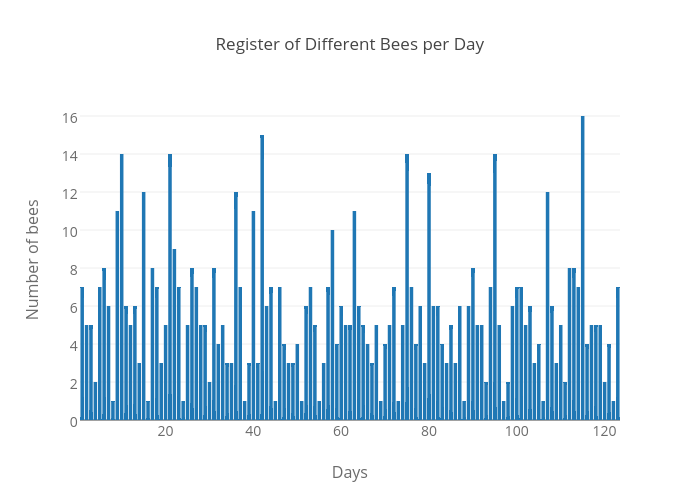
\includegraphics[width=400px]{differentBeesPerdayClean.png}%
\caption{Different Bees Per Day}%
\end{figure}

%


\begin{figure}[h!]%
\centering%
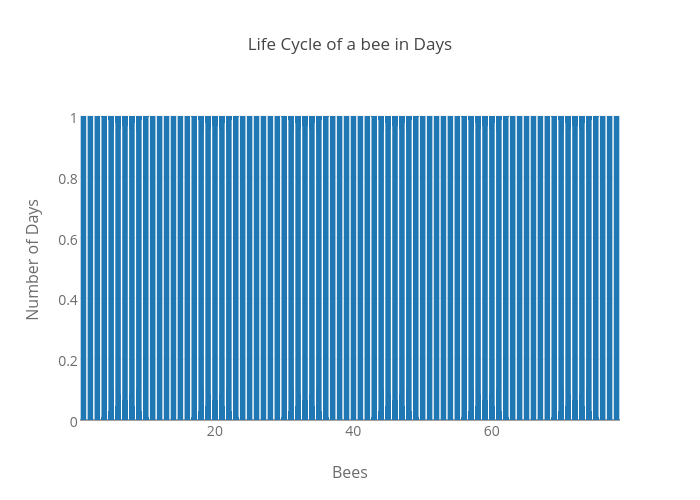
\includegraphics[width=400px]{beeLifeCycleClean.png}%
\caption{Bee Life cycle in days}%
\end{figure}

%


\begin{figure}[h!]%
\centering%
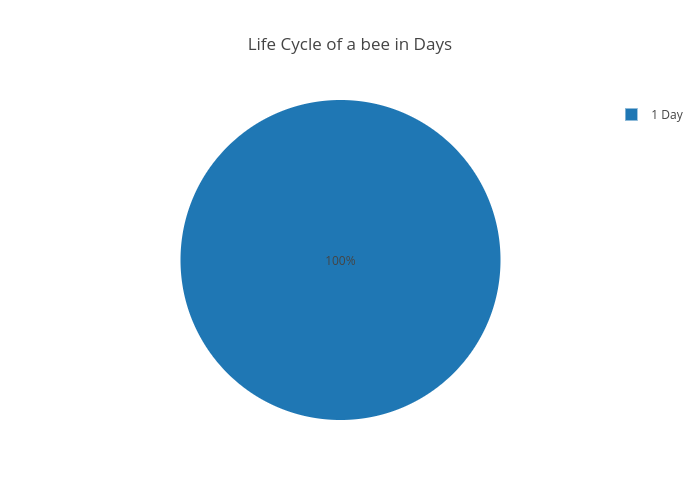
\includegraphics[width=400px]{pieBeeLifeCycleClean.png}%
\caption{Bee Life cycle in days}%
\end{figure}

%
\subsection*{Analysis of Activity per Hour}%


\begin{figure}[h!]%
\centering%
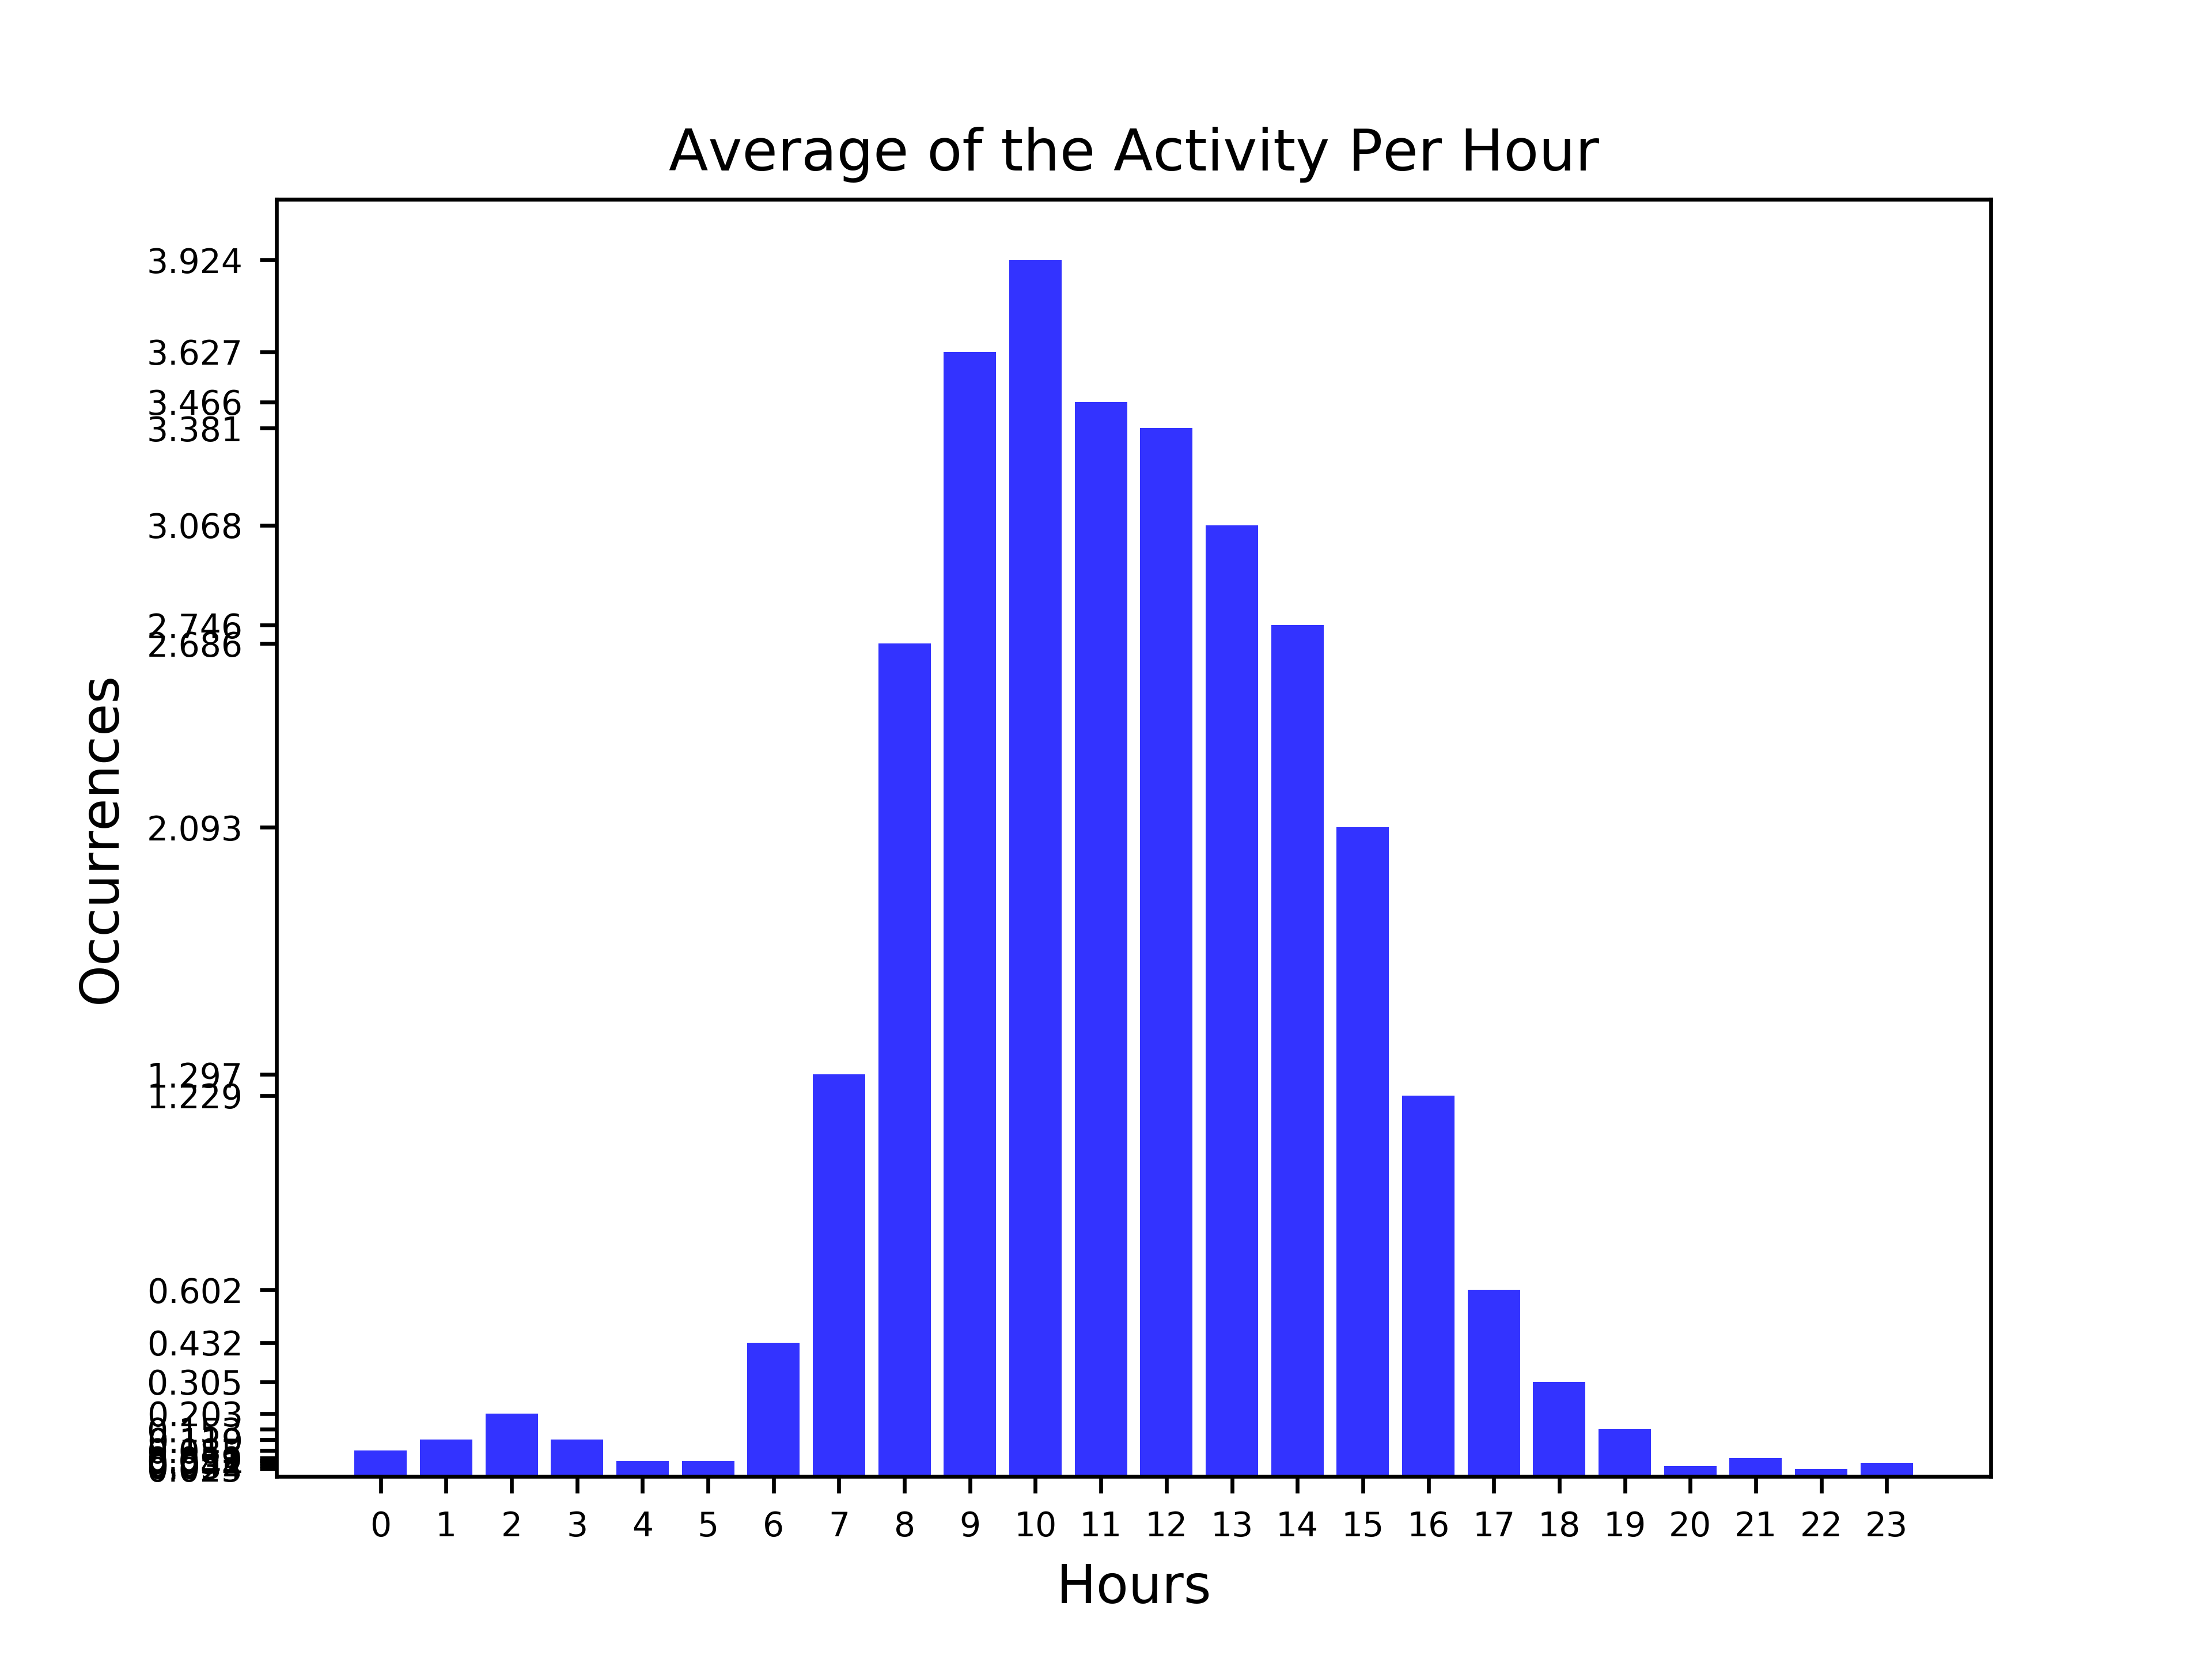
\includegraphics[width=400px]{histogramClean.png}%
\caption{Histogram of frequencies per hour}%
\end{figure}

%


\begin{figure}[h!]%
\centering%
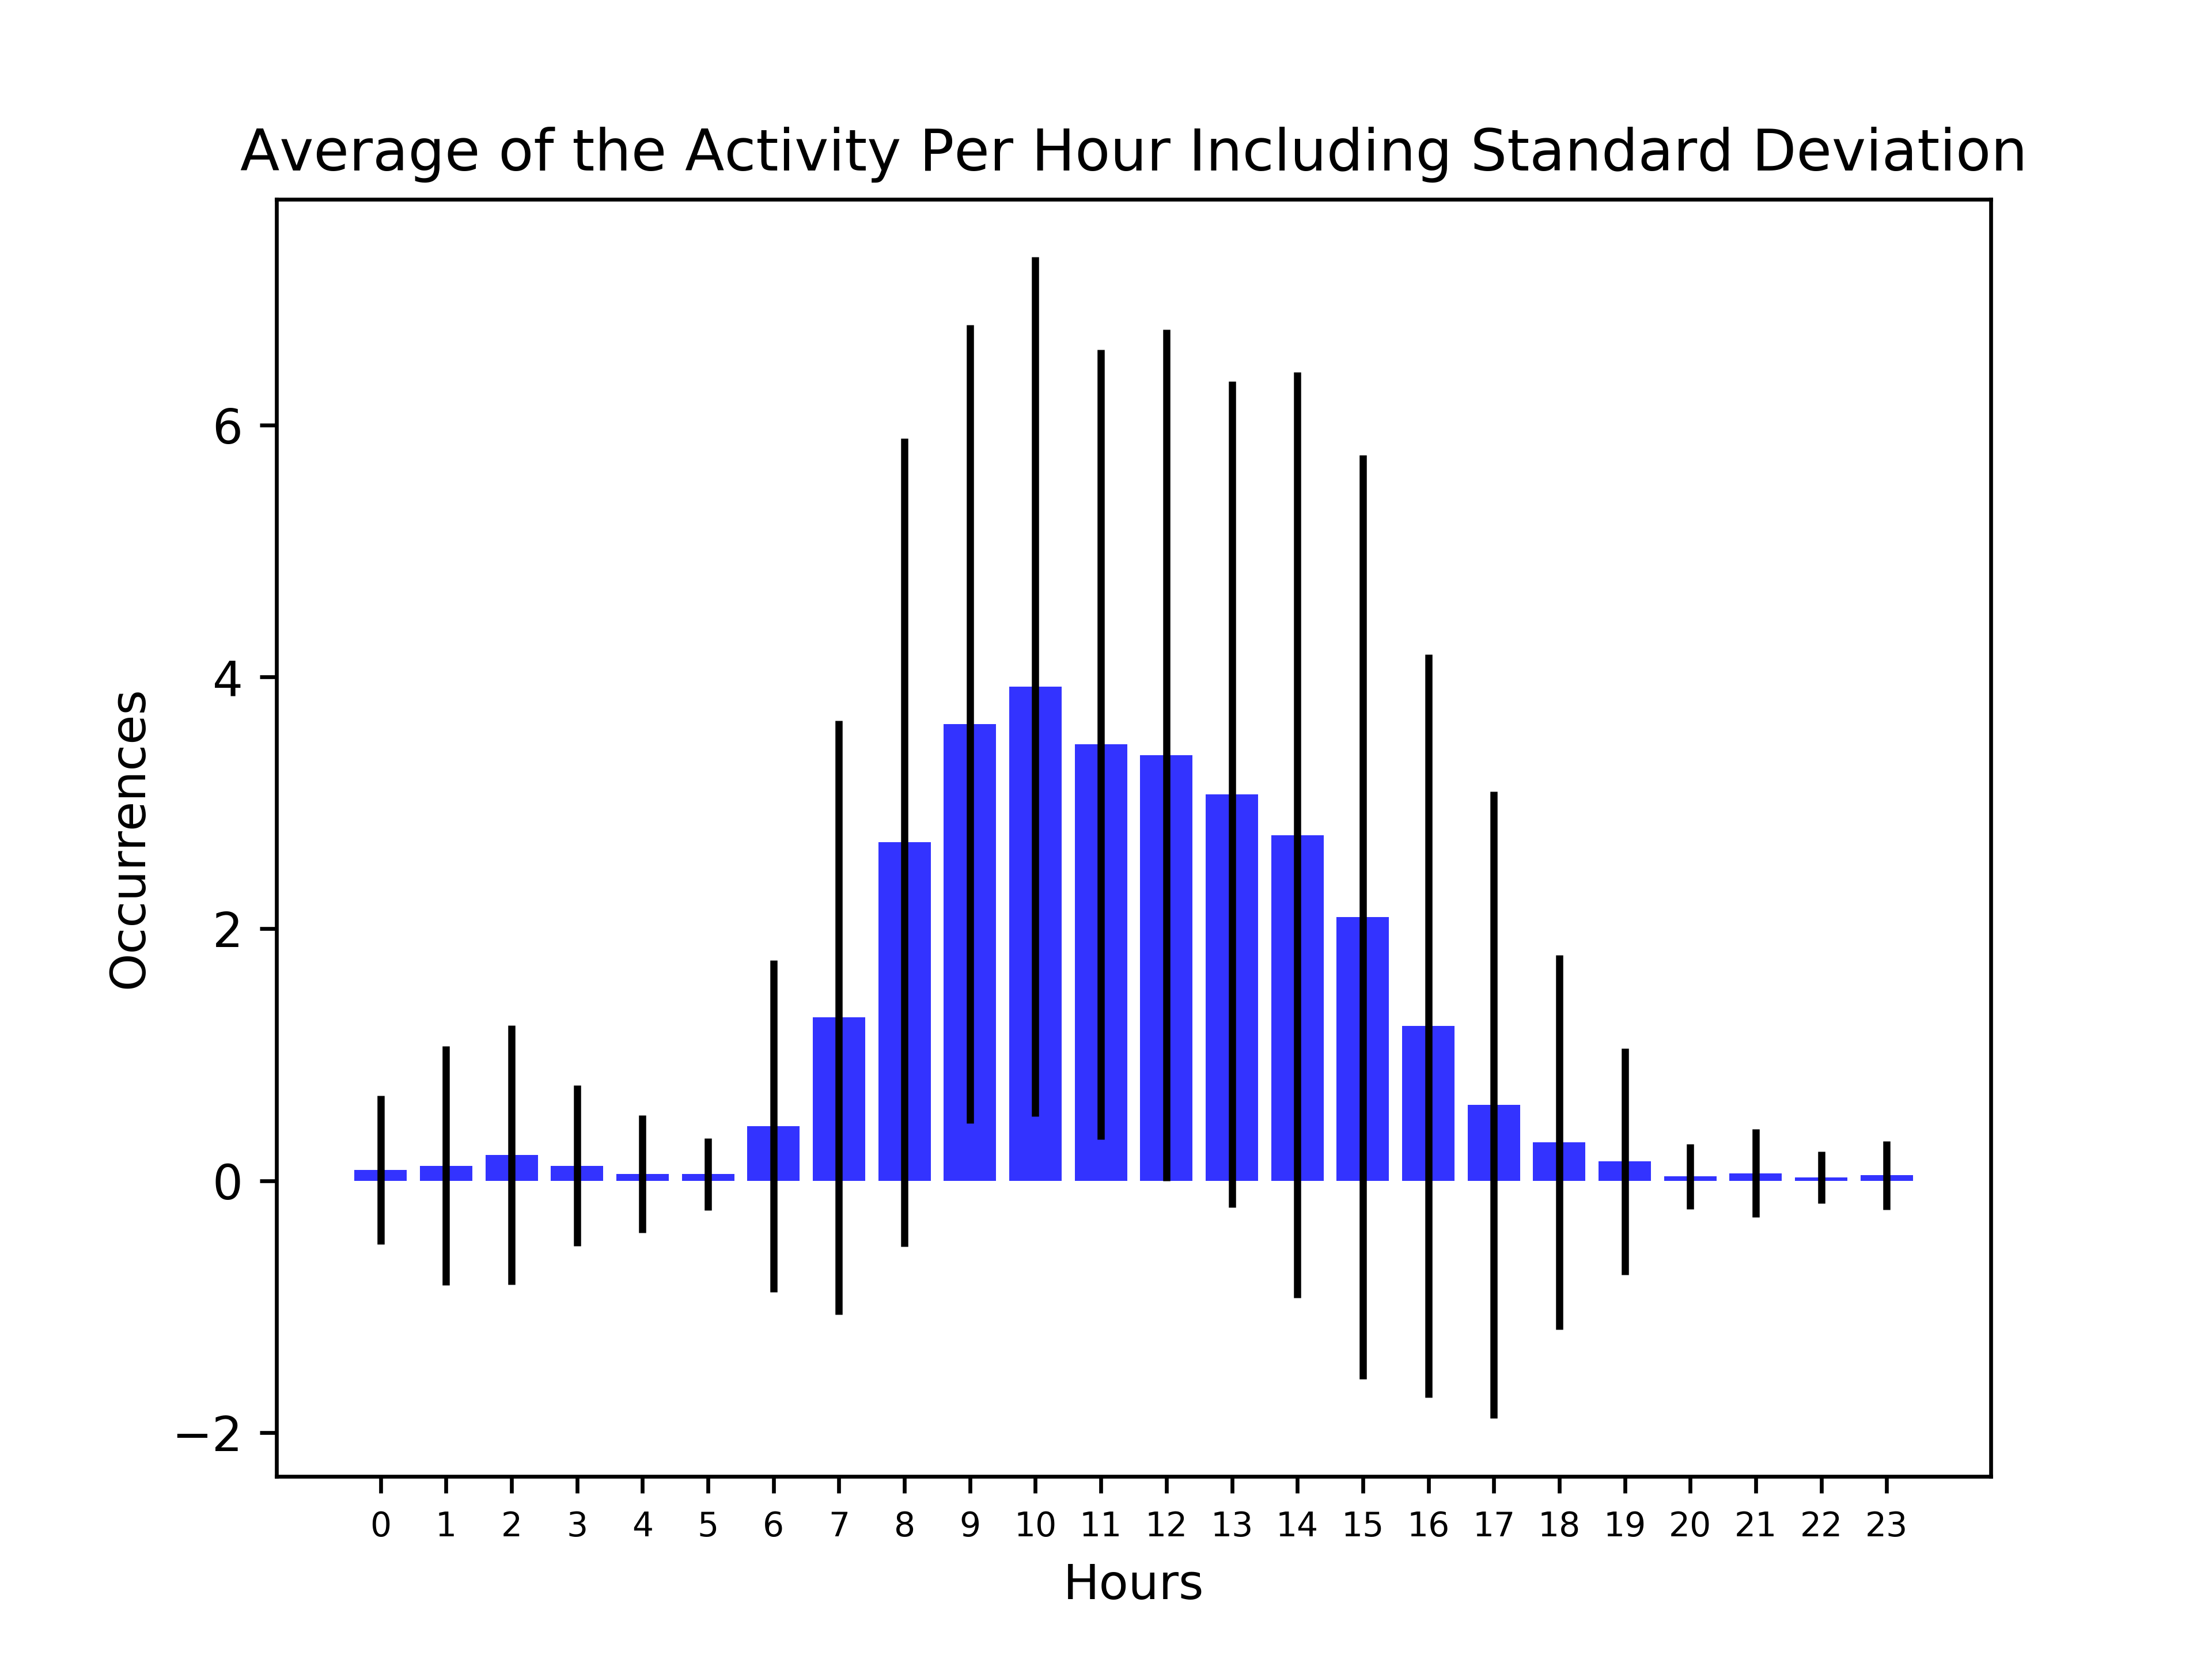
\includegraphics[width=400px]{histogramStdClean.png}%
\caption{Histogram of frequencies per hour. It includes standard deviation}%
\end{figure}


\chapterimage{head5.jpg} % Chapter heading image
\chapter{Analysis of Foraging Behavior}

\end{document}